% Explanation-focused replacement fragment; source/score hashes are in
% artifacts/roboboat-transfer-accuracy-2026-10-02/explanation-transfer-results.json.
\subsection{Evidence-calibrated explanations across land and marine domains}
\label{sec:marine-temporal-evidence}

The marine evaluation tests whether the paper's central explanation behaviors
transfer to autonomous surface navigation: reporting supported claims,
communicating useful available information, and withholding conclusions when
required evidence is missing. The question is how accurately the explanation
tracks its evidence, rather than how successfully the vessel navigates. A
correctly calibrated answer can diagnose an observed violation or state that
completion is unknown; neither is a navigation-performance score.

We apply the same evidence-contract principle through marine-specific task
contracts, odometry adapters and temporal computations. Land commands, motion
and execution history govern supported diagnostic claims. Marine action status,
adjacent pose/velocity measurements and a sampled five-second interval govern
physical-completion claims. L0, L1 and L2 remove information from the same
recording, testing whether explanation specificity grows with evidence while
unsupported completion and causal claims remain withheld.

Existing evaluated answers provide direct evidence of explanation quality
(Table~\ref{tab:marine-explanation-quality}). Across five development recordings
in three approach clusters, the marine calibrated implementation achieved
15/15 successful answers and 60/60 required information units. All 15 answers
were assessed as supporting their inventoried claims and preserving causal
limitations. In a separate explicit-contact replay over two existing recordings,
all six answers passed development support/coverage criteria: 116/116 reviewed
claim instances were supported, 24/24 common information units were communicated,
and both answerable positive sampled-compliance intervals were explained.
The banks remain separate; levels, claims and judge passes add no independent
configuration N. The first bank uses project sentence inventories; its later
incomplete atomic reassessment does not replace these scores.

The timeline/evidence-ladder figures show what those results mean. In the
violation example (Fig.~\ref{fig:marine-violation-explanation}), the answer changes
from unknown interval completion at L0 to an adjacent measurement at L1, then
identifies a witnessed within-dwell yaw-rate violation at L2. It invents no
physical cause. In the positive example (Fig.~\ref{fig:marine-positive-explanation}),
L2 reports that all 251 observed kinematic/hull samples met the interval
requirements, while retaining unknown contact and unproved continuous compliance.
A later position crossing is outside that interval and cannot reverse its
sampled-compliance statement. The excerpts are verbatim evaluated answers,
rather than newly written ideal responses.

These results support transfer of the core calibration behavior to a practically
motivated surface-vessel task, consistent with the land study's supported-diagnosis,
coverage and evidential-restraint objectives. They do not estimate equal
land/marine accuracy or superiority over another method. The evaluated marine
condition uses deterministic language and domain-specific computations, rather
than an unchanged transfer of the full land pipeline. Labels are automated
agent-assessed development evidence with possible correlated error, not human
validation. Existing docking-policy explanations already use surrogate
models~\cite{gjarum2021docking}; the transferred behavior here concerns support
for execution-completion claims. The demonstrated application is simulated;
real-water accuracy and broader generalization remain to be tested.

\begin{table}[t]
\caption{Observed marine explanation quality in separate inspected development
banks. Successful answers require supported inventoried claims, required-unit
coverage and preserved limitations. These are automated support assessments,
not population error bounds or a pooled domain-comparison estimate.}
\label{tab:marine-explanation-quality}
\centering\small
\begin{tabular}{lrr}
\hline
Evaluated bank & Answers & Required units \\
\hline
Five-record violation bank & 15/15 & 60/60 \\
Two-record contact replay & 6/6 & 24/24 \\
\hline
\end{tabular}
\end{table}

\begin{figure*}[t]
\centering
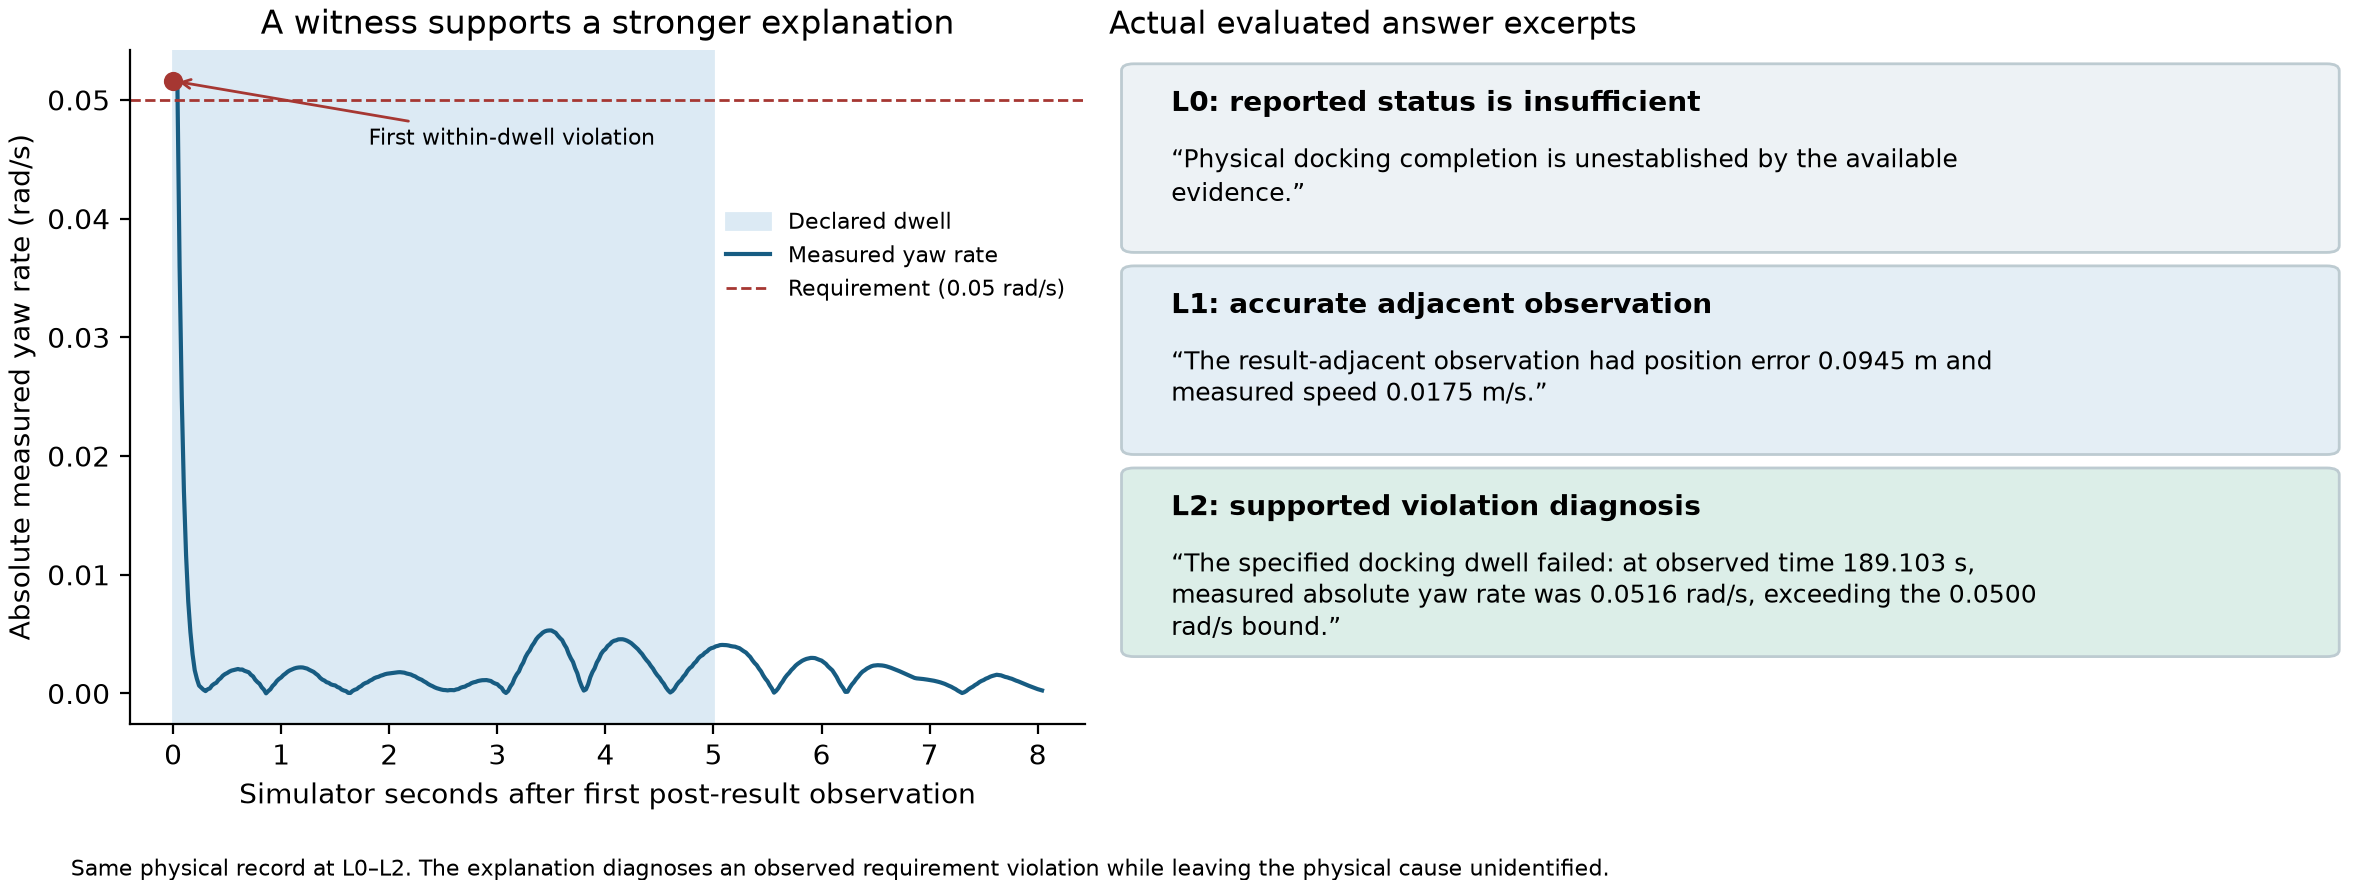
\includegraphics[width=\textwidth]{../artifacts/roboboat-transfer-accuracy-2026-10-02/marine-violation-evidence-ladder.png}
\caption{Evidence-sensitive diagnosis in the scored direct-route recording.
The same-record answer moves from withholding interval completion to adjacent
measurements and then a supported yaw-rate-violation witness. Text excerpts are
verbatim from evaluated answers. Shading is the fixed dwell; time zero is its
first post-result observation. The complete answers retain causal uncertainty.}
\label{fig:marine-violation-explanation}
\end{figure*}

\begin{figure*}[t]
\centering
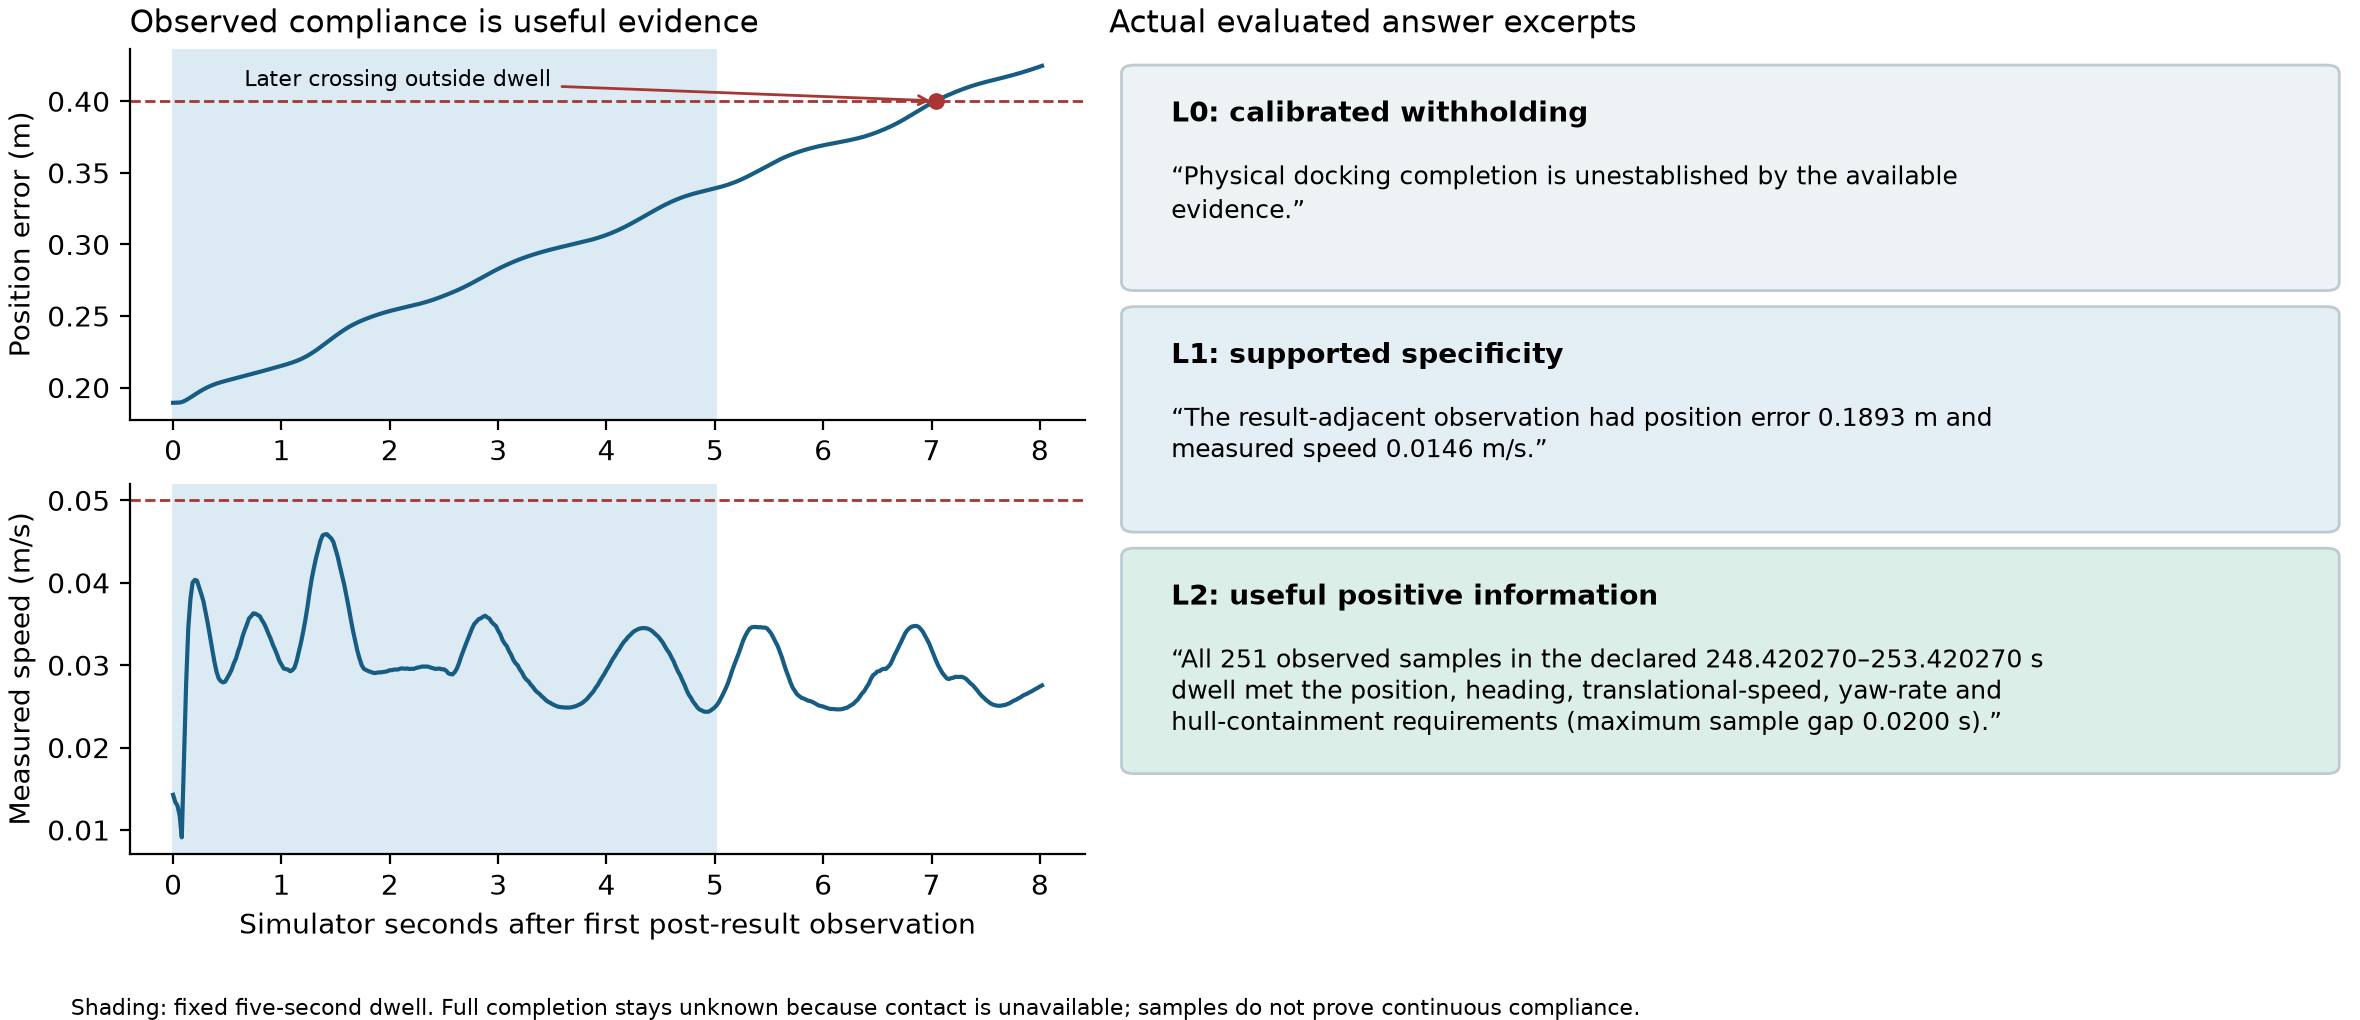
\includegraphics[width=\textwidth]{../artifacts/roboboat-transfer-accuracy-2026-10-02/marine-positive-evidence-ladder.png}
\caption{Useful positive evidence without an unsupported completion claim.
The known-route contact-replay answer communicates sampled kinematic/hull
compliance across the shaded fixed dwell. Its full text retains unknown contact
and continuous-time limits. The later position crossing is outside the interval
and does not falsify earlier sampled compliance. Excerpts are verbatim evaluated
answers; plotted lines interpolate samples for display, not physical proof.}
\label{fig:marine-positive-explanation}
\end{figure*}

% Optional supplementary figure if the main-paper page allocation is tight.
\begin{figure*}[t]
\centering
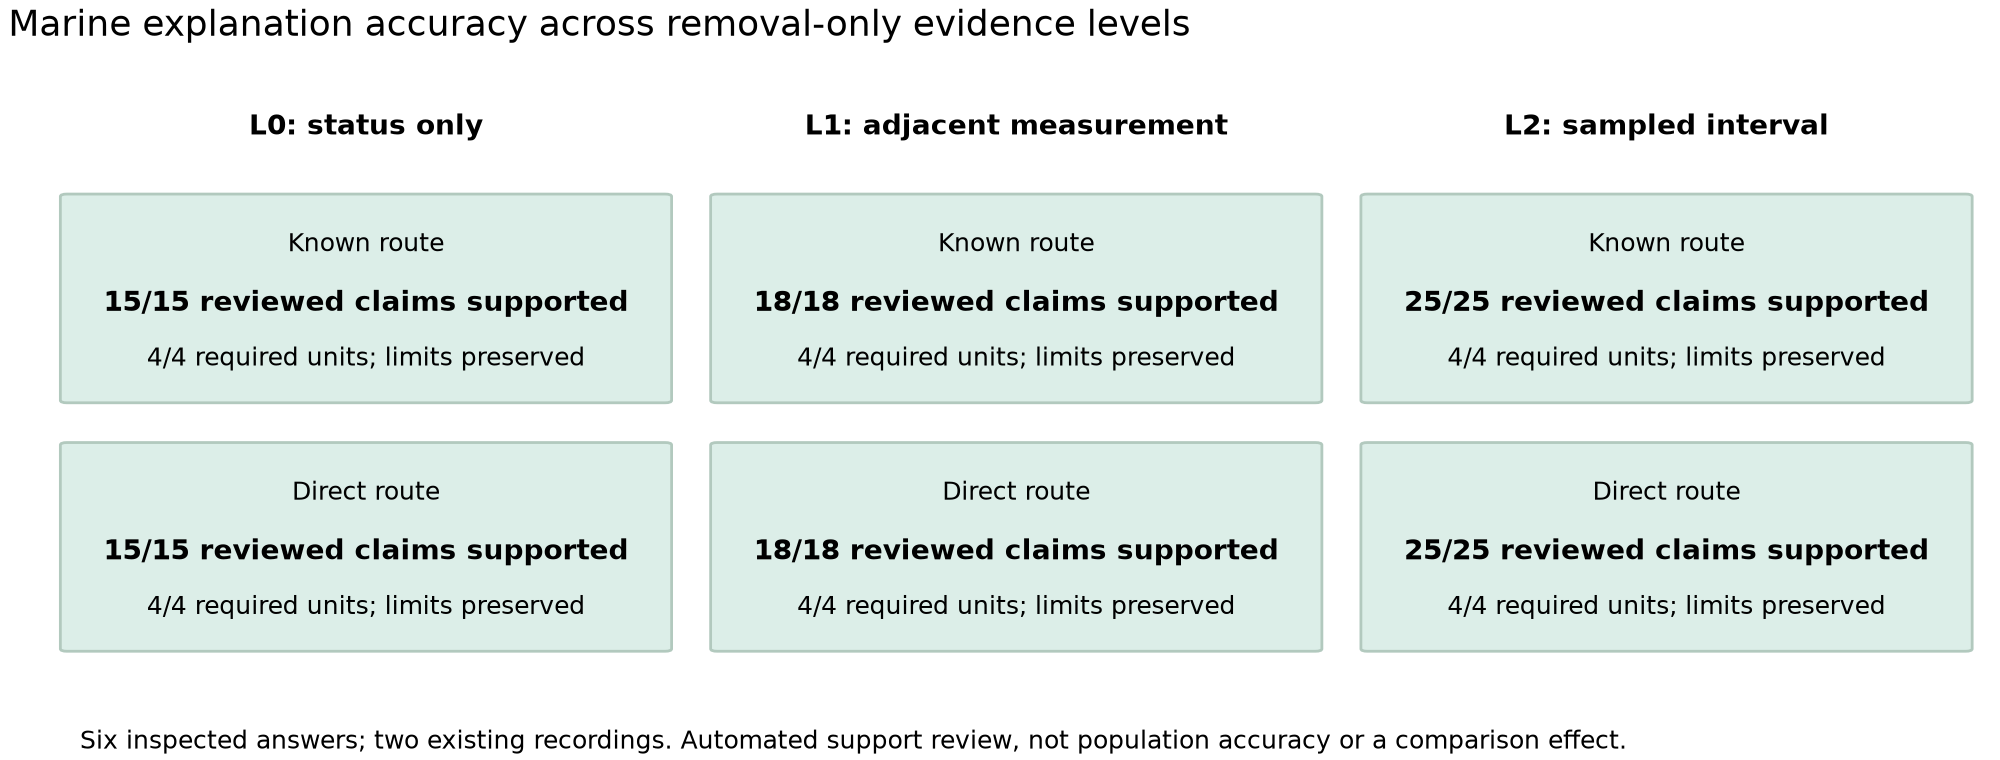
\includegraphics[width=\textwidth]{../artifacts/roboboat-transfer-accuracy-2026-10-02/marine-explanation-quality.png}
\caption{All six calibrated answers in the closed explicit-contact replay.
Each cell reports reviewed claim support and required-unit coverage for one
recording/evidence level. The full answers preserve limitations. Claim counts
are annotation denominators, not independent observations or an objective to
maximize. The five-record bank and the replay are not pooled.}
\label{fig:marine-explanation-support-matrix}
\end{figure*}
